\documentclass[a4paper, 12pt]{article}

%%% SST LAB PROTOCOLL PREAMBLE
%%% 2019
%%%%%%%%%%%%%%%%%%%%%%%%%%%%%%%


%%% PACKAGES
%%%%%%%%%%%%%%%%%%%%%%%%%%%

\usepackage[ngerman]{babel}

\usepackage[utf8]{inputenc}
\usepackage{amsmath}
\usepackage{pgfplots}
\usepackage{tikz}
\usepackage[many]{tcolorbox}
\usepackage{graphicx}
\graphicspath{ {./graphics/} }
\usepackage{pdfpages}
\usepackage{dashrule}
\usepackage{float}
\usepackage{siunitx}
\usepackage{booktabs}
\usepackage[version=4]{mhchem}

%%% DOCUMENT GEOMETRY
%%%%%%%%%%%%%%%%%%%%%%%%%%%

\usepackage{geometry}
\geometry{
 a4paper,
 total={0.6180339887498948\paperwidth,0.6180339887498948\paperheight},
 top = 0.1458980337503154\paperheight,
 bottom = 0.1458980337503154\paperheight
 }
\setlength{\jot}{0.013155617496424828\paperheight}
\linespread{1.1458980337503154}

\setlength{\parskip}{0.013155617496424828\paperheight} % paragraph spacing


%%% COLORS
%%%%%%%%%%%%%%%%%%%%%%%%%%%

\definecolor{red1}{HTML}{f38181}
\definecolor{yellow1}{HTML}{fce38a}
\definecolor{green1}{HTML}{95e1d3}
\definecolor{blue1}{HTML}{66bfbf}
\definecolor{hsblue}{HTML}{00b1db}
\definecolor{hsgrey}{HTML}{afafaf}

%%% CONSTANTS
%%%%%%%%%%%%%%%%%%%%%%%%%%%
\newlength{\smallvert}
\setlength{\smallvert}{0.0131556\paperheight}


%%% COMMANDS
%%%%%%%%%%%%%%%%%%%%%%%%%%%

% differential d
\newcommand*\dif{\mathop{}\!\mathrm{d}}

% horizontal line
\newcommand{\holine}[1]{
  	\begin{center}
	  	\noindent{\color{hsgrey}\hdashrule[0ex]{#1}{1pt}{3mm}}\\%[0.0131556\paperheight]
  	\end{center}
}

% mini section
\newcommand{\minisec}[1]{ \noindent\underline{\textit {#1} } \\}

% quick function plot
\newcommand{\plotfun}[3]{
  \vspace{0.021286\paperheight}
  \begin{center}
    \begin{tikzpicture}
      \begin{axis}[
        axis x line=center,
        axis y line=center,
        ]
        \addplot[draw=red1][domain=#2:#3]{#1};
      \end{axis}
    \end{tikzpicture}
  \end{center}
}

% box for notes
\newcommand{\notebox}[1]{

\tcbset{colback=white,colframe=red1!100!black,title=Note!,width=0.618\paperwidth,arc=0pt}

 \begin{center}
  \begin{tcolorbox}[]
   #1 
  \end{tcolorbox}
 
 \end{center} 
 
}

% box for equation
\newcommand{\eqbox}[2]{
	
	\tcbset{colback=white,colframe=hsblue!100!black,title=,width=#2,arc=0pt}
	
	\begin{center}
		\begin{tcolorbox}[ams align*]
				#1
		\end{tcolorbox}
		
	\end{center} 
	
}

% END OF PREAMBLE

%%%%%%%%%%%%%%%%%%%%%%%%%%%%%%%%%%%%%

\begin{document}

%%%%%%%%%%%%%%%%%%%%%%%%%%%%%%%%%%%%%
  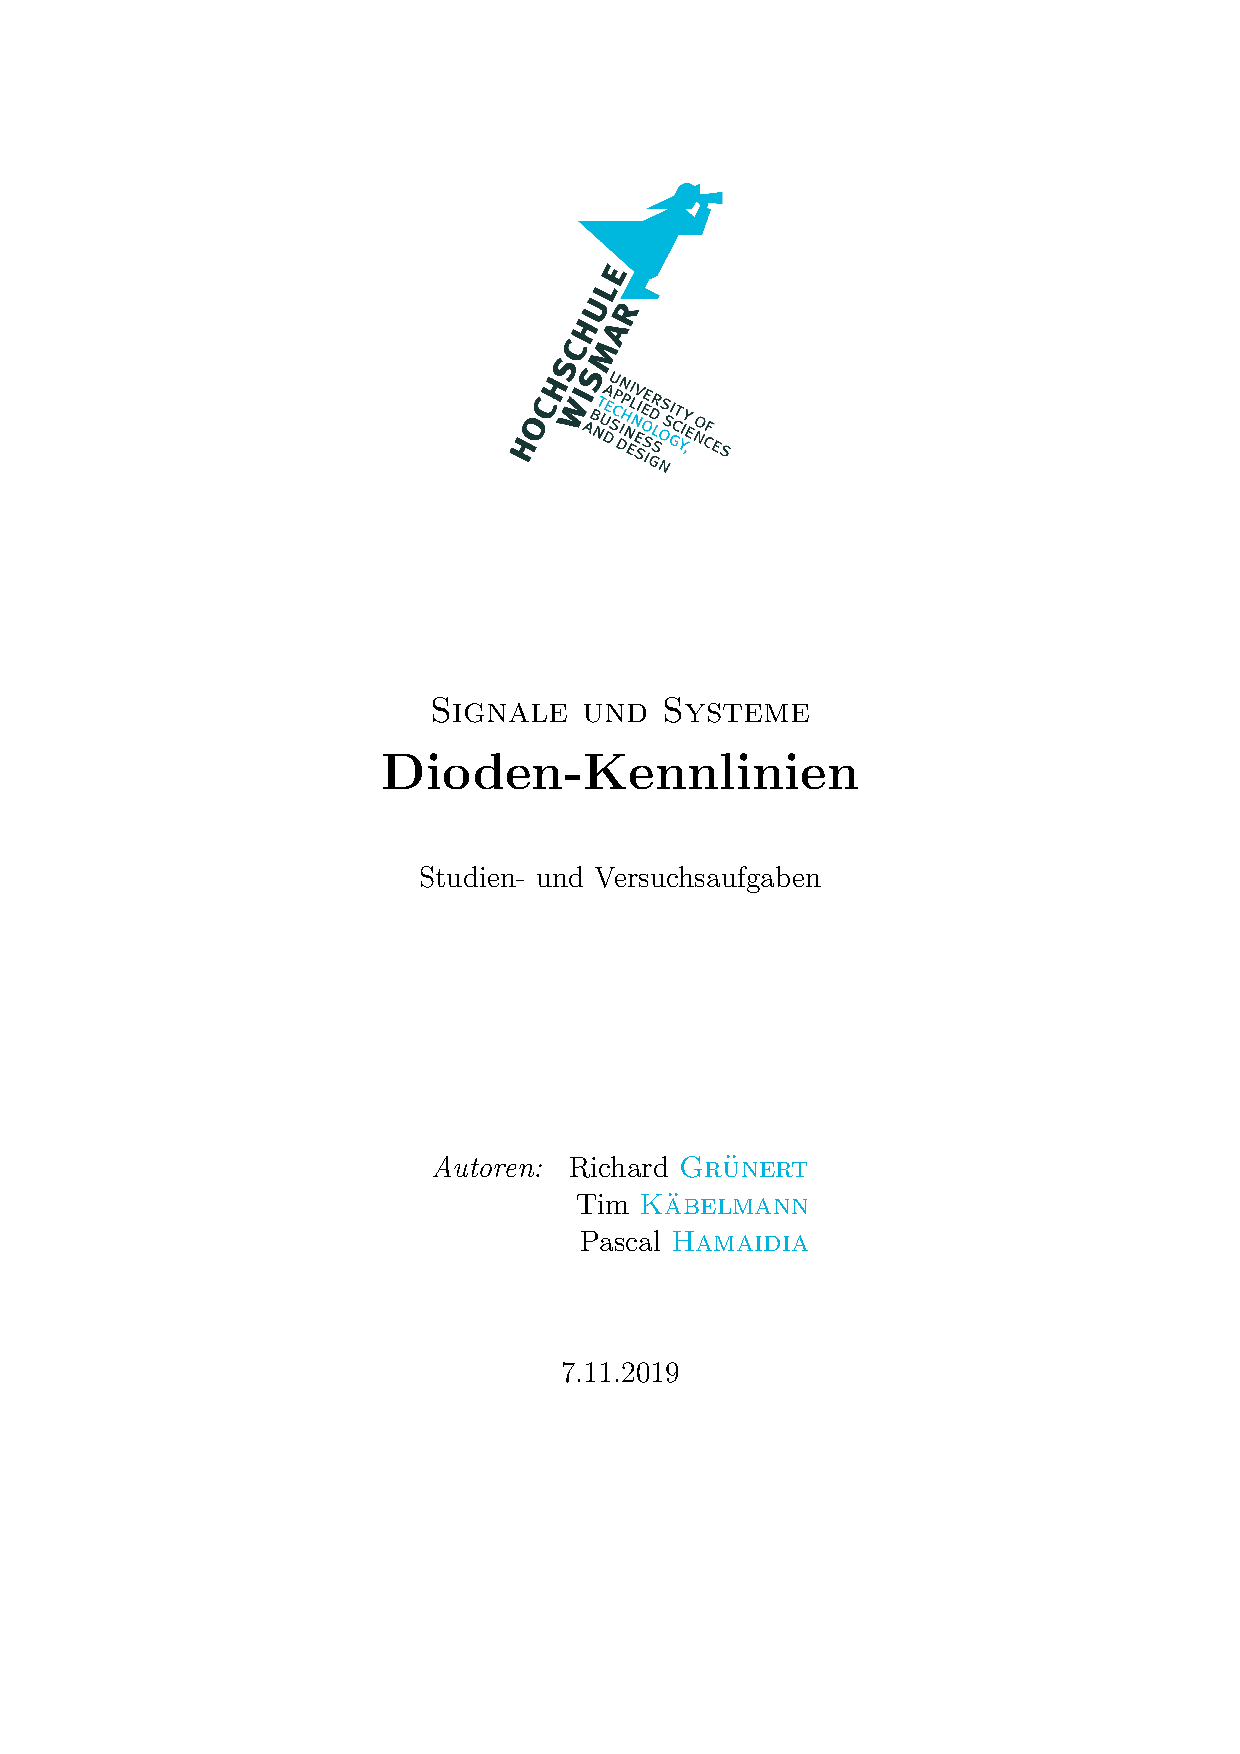
\includepdf{./titlepage/titlepage.pdf}
  \clearpage
  \setcounter{page}{1}
%%%%%%%%%%%%%%%%%%%%%%%%%%%%%%%%%%%%%

\section{Vorbereitungsaufgaben}

% 1.1
\subsection{Aufbau und Wirkungsweise eines pn-Übergangs}
Dotiert man einen Halbleiterkristall (z.B. \ce{Si} oder \ce{Ge}) mit Fremdatomen, 


% 1.1
\subsection{Aufbau und Wirkungsweise einer Diode}
Die elektrischen Eigenschaften des pn-Übergangs können technisch ausgenutzt werden, um eine \emph{Diode} zu realisieren. Der Stromfluss durch den pn-Übergang ist von der Polarität der über ihn angelegten Spannung abhängig. Man definiert daher die Orientierung der Diode in \emph{Sperr-} und \emph{Durchlassrichtung}.

% 1.1
\subsection{Z- und Schottky-Dioden}

% 1.1
\subsection{Spannungsstabilisierungsschaltung}

% 1.1
\subsection{Dimensionierung des Vorwiderstands}

% 1.1
\subsection{Diodenkennlinie}

% 1.1
\subsection{Diodengrenzwerte}


% 2
%%%%%%%%%%%%%%%%%%%%%%%%%%%%%%%%%%%%%
\section{Versuchsaufgaben}

% 2.1
\subsection{Diodenkennline BY500}

% 2.2
\subsection{Diodenkennline ZY5,6}

% 2.3
\subsection{Z-Spannung und differentieller Widerstand}

% 2.4
\subsection{Spannungsstabilisierung bei veränderlicher Eingangsspannung}

% 2.5
\subsection{Spannungsstabilisierung bei veränderlichem Laststrom}

\end{document}
